\begin{figure}
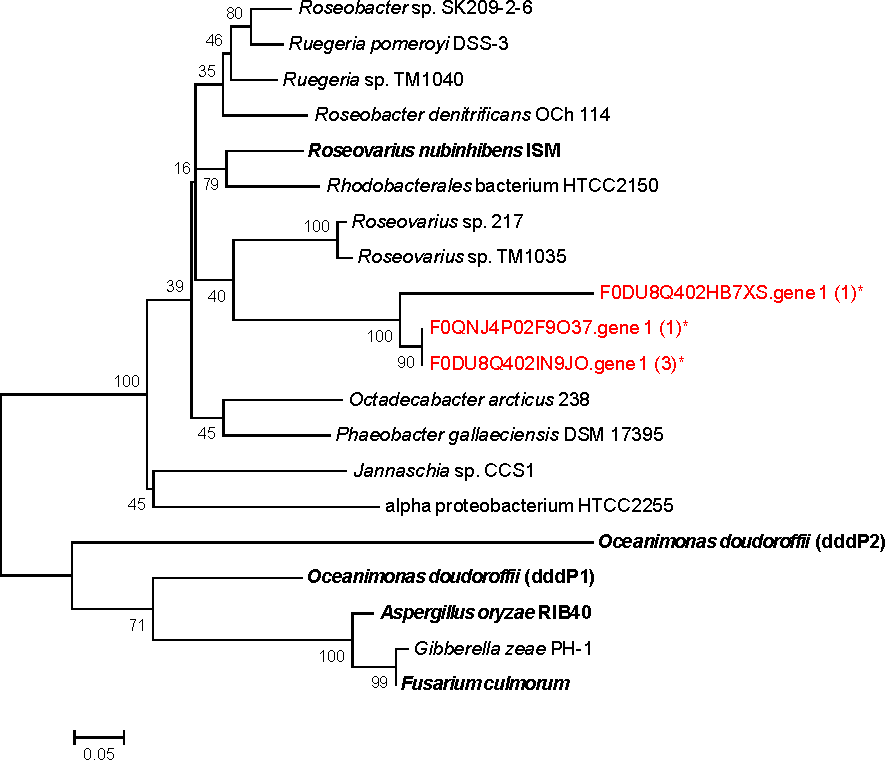
\includegraphics{orglake_figures/dddP_tree.pdf}
\caption[Phylogenetic tree of DddP DMSP lyase homologues]{Phylogenetic tree of DddP DMSP demethylase homologues. The tree was computed from a 129 amino acid C-terminal region using the neighbour-joining algorithm. Organic Lake sequences from this study are shown in red and marked with an asterisk (*). Numbers in parentheses are counts of sequences that clustered with the Organic Lake homologue shown in the tree with 90\% amino acid identity. Sequences with confirmed DMSP lyase activity are shown in bold. Accession numbers from top to bottom are: ZP\_01755203, YP\_167522, YP\_613011, YP\_682809, EAP77700, ZP\_01741265, ZP\_01036399, ZP\_01881042, ZP\_05063825, AFO91571, YP\_509721, ZP\_01448542, AEQ39103, AEQ39091, XP\_001823911, XP\_389272 and ACF19795.}
\label{fig:dddP_tree}

\end{figure}
